\documentclass[aspectratio=169]{beamer}
\mode<presentation> {
%\usetheme{default}
%\usetheme{AnnArbor}
%\usetheme{Antibes}
%\usetheme{Bergen}
%\usetheme{Berkeley}
%\usetheme{Berlin}
%\usetheme{Boadilla}
%\usetheme{CambridgeUS}
%\usetheme{Copenhagen}
%\usetheme{Darmstadt}
%\usetheme{Dresden}
%\usetheme{Frankfurt}
%\usetheme{Goettingen}
%\usetheme{Hannover}
%\usetheme{Ilmenau}
%\usetheme{JuanLesPins}
%\usetheme{Luebeck}
%\usetheme{Madrid}
%\usetheme{Malmoe}
%\usetheme{Marburg}
%\usetheme{Montpellier}
%\usetheme{PaloAlto}
%\usetheme{Pittsburgh}
%\usetheme{Rochester}
%\usetheme{Singapore}
%\usetheme{Szeged}
\usetheme{Warsaw}
}
\usepackage{graphicx} % Allows including images
\usepackage{booktabs} % Allows the use of \toprule, \midrule and \bottomrule in tables
\usepackage{textcomp}
\usepackage{tikz}
\usetikzlibrary{shapes}
\usepackage{amsfonts,amsmath}
\usepackage{mathrsfs}
\usepackage{color}
\usepackage{epsfig}
\usepackage{comment}
\usepackage[T1]{fontenc}
\usepackage{mathtools}          %loads amsmath as well
\usepackage{textcomp}%fixed - problem in listing
\usepackage{listings}

\definecolor{mygreen}{rgb}{0,0.6,0}
\definecolor{mygray}{rgb}{0.5,0.5,0.5}
\definecolor{mymauve}{rgb}{0.58,0,0.82}

\lstset{ 
  backgroundcolor=\color{white},   % choose the background color; you must add \usepackage{color} or \usepackage{xcolor}; should come as last argument
  basicstyle=\footnotesize,        % the size of the fonts that are used for the code
  breakatwhitespace=false,         % sets if automatic breaks should only happen at whitespace
  breaklines=true,                 % sets automatic line breaking
  captionpos=b,                    % sets the caption-position to bottom
  commentstyle=\color{mygreen},    % comment style
  deletekeywords={...},            % if you want to delete keywords from the given language
  escapeinside={\%*}{*)},          % if you want to add LaTeX within your code
  extendedchars=true,              % lets you use non-ASCII characters; for 8-bits encodings only, does not work with UTF-8
  %firstnumber=1000,                % start line enumeration with line 1000
  frame=single,	                   % adds a frame around the code
  keepspaces=true,                 % keeps spaces in text, useful for keeping indentation of code (possibly needs columns=flexible)
  keywordstyle=\color{blue},       % keyword style
  %language=Octave,                 % the language of the code
  morekeywords={*,...},            % if you want to add more keywords to the set
  numbers=left,                    % where to put the line-numbers; possible values are (none, left, right)
  numbersep=5pt,                   % how far the line-numbers are from the code
  numberstyle=\tiny\color{mygray}, % the style that is used for the line-numbers
  rulecolor=\color{black},         % if not set, the frame-color may be changed on line-breaks within not-black text (e.g. comments (green here))
  showspaces=false,                % show spaces everywhere adding particular underscores; it overrides 'showstringspaces'
  showstringspaces=false,          % underline spaces within strings only
  showtabs=false,                  % show tabs within strings adding particular underscores
  %stepnumber=2,                    % the step between two line-numbers. If it's 1, each line will be numbered
  stringstyle=\color{mymauve},     % string literal style
  tabsize=2,	                   % sets default tabsize to 2 spaces
  %title=\lstname                   % show the filename of files included with \lstinputlisting; also try caption instead of title
 %caption=\lstname
}


\definecolor{light-gray}{gray}{0.70}

\def\ArtWork#1{\noindent\hfill\epsfbox{#1}\hfill}%
\def\MyArtWork#1#2{\noindent\centerline{\epsfxsize=0.22\hsize\epsfbox{#1}\hspace{1in}\epsfxsize=0.22\hsize\epsfbox{#2}}}

\newcommand{\tcbr}{\textcolor{black}}
\newcommand{\pr}{\textsf{Pr}}
\newcommand{\sym}[1]{{\sf #1}}
\newcommand{\la}{\leftarrow}
\newcommand{\ra}{\rightarrow}
\newcommand{\gf}{\mbox{\it GF}}
\newcommand{\rand}{\stackrel{*}\leftarrow}
\newcommand{\torand}{\stackrel{*}{\rightarrow}}
\newcommand{\randu}{\stackrel{\$}{\leftarrow}}
\renewcommand{\a}{\alpha}
\renewcommand{\b}{\beta}
\renewcommand{\th}{^{\mathrm{th}}}
\newcommand{\tor}{\Rightarrow}
\newcommand{\tol}{\Leftarrow}
\newcommand{\tolr}{\Leftrightarrow}
\newcommand{\tcirc}[1] {\mbox{$\stackrel{\circ}{\mbox{#1}}$}}
\newcommand{\emstr}{\mbox{$\langle \rangle$}}
\newcommand{\pf}{\noindent{\bf Proof. }}
\newcommand{\s}{\{0,1\}}
\newcommand{\tx}{\textsf}
\newcommand{\too}{\Longrightarrow}
\renewcommand{\th}{^{\mathrm{th}}}
\newcommand{\eqL}{\stackrel{\mathcal{L}}{=}}
\newcommand{\Perm}{\mathrm{Perm}}
\newcommand{\Func}{\mathrm{Func}}
\newcommand{\LPerm}{\mathrm{Perm}^{\mathrm{LP}}}

\newcommand{\E}{\mathbf{E}}
\newcommand{\Dec}{\mathbf{D}}


\newcommand{\tcr}{\textcolor{red}}
\newcommand{\ttH}{{\tt H}}
\newcommand{\ttf}{{\tt f}}
\newcommand{\tth}{{\tt h}}
\newcommand{\ttR}{{\tt R}}
\newcommand{\ttS}{{\tt S}}
\newcommand{\ttX}{{\tt X}}
\newcommand{\ttY}{{\tt Y}}
\newcommand{\ttP}{{\tt P}}
\newcommand{\ttF}{{\tt F}}
\newcommand{\ttG}{{\tt G}}

\newcommand{\ff}{\mathbb{F}_{2^n}}

\newcommand{\iid}{\stackrel{\mathrm{iid}}{\sim}}
\newcommand{\veceq}{\stackrel{\mathrm{iid}}{\sim}}
\newcommand{\polya}{P$\acute{o}$lya}

\newcommand{\BPP}{\mathcal{BPP}}
\newcommand{\IP}{\mathcal{IP}}
\newcommand{\NP}{\mathcal{NP}}
\newcommand{\M}{\mathcal{M}}
\newcommand{\K}{\mathcal{K}}
\newcommand{\calO}{\mathcal{O}}
\newcommand{\T}{\mathcal{T}}
\newcommand{\A}{\mathcal{A}}
\newcommand{\D}{\mathcal{D}}


\newcommand{\law}{\stackrel{\mathcal{L}}{=}}

\DeclarePairedDelimiter{\norm}{\lVert}{\rVert} 
\DeclarePairedDelimiter\Floor\lfloor\rfloor
\DeclarePairedDelimiter\Ceil\lceil\rceil


%----------------------------------------------------------------------------------------
%	TITLE PAGE
%----------------------------------------------------------------------------------------
\usebackgroundtemplate{\tikz\node[opacity=0.04]{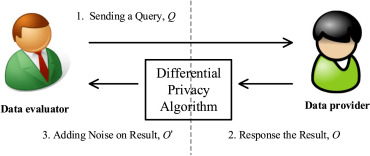
\includegraphics[width=\paperwidth,height=\paperheight]{background.jpg}};}

\title{A survey on Differential Privacy} % The short title appears at the bottom of every slide, the full title is only on the title page
\author[Sarbajit Ghosh]{\large Sarbajit Ghosh}
% Your name
\institute[ISI, Kolkata] {
\textcolor{blue}{  Under Guidence of Dr. Srimanta Bhattacharya  \\ \vspace*{1 pt}
Indian Statistical Institute, Kolkata} 
}
\titlegraphic{
\includegraphics[width=1cm]{isi.png} }
\date{\vspace{-5ex}} % Date, can be changed to a custom date
\begin{document}
	\tikzstyle{decision} = [diamond, draw, text width=4.5em, text badly centered, node distance=3cm, inner sep=0pt]
	\tikzstyle{block} = [rectangle, draw,  text width=1.8em, text centered,  minimum height=1.8em]
	\tikzstyle{bl} = [rectangle, draw,  text width=1.8em, text centered,  minimum height=1.8em, minimum width=3.8em]
	\tikzstyle{block5} = [rectangle, draw, fill=magenta!20, text width=1.8em, text centered,  minimum height=1.8em]
	\tikzstyle{block6} = [rectangle, draw,  fill=cyan!40!white, text width=1.8em, text centered,  minimum height=1.8em, minimum width=3.8em]
	\tikzstyle{wideblock} = [rectangle, draw,  fill=cyan!40!white, text width=1.8em, text centered,  minimum height=1.8em, minimum width=8.8em]
	\tikzstyle{line} = [draw, -latex]
	\tikzstyle{XOR} = [draw, circle]
	\tikzstyle{cloud} = [draw, ellipse, node distance=3cm, minimum height=2em]
\tikzstyle{block} = [rectangle, draw,  text width=2em, text centered,  minimum height=2.5em]

\tikzstyle{block0} = [rectangle, draw,  text width=2.2em, text centered,  minimum height=1.8em]
\tikzstyle{block1} = [rectangle, draw,  fill=blue, text width=0.2em, text centered,  minimum height=0.2em]
\tikzstyle{block2} = [rectangle, draw,  text width=1.5em, text centered,  minimum height=1.5em]
\tikzstyle{block3} = [rectangle, draw,  text width=4em, text centered,  minimum height=3em]
\tikzstyle{block4} = [rectangle, draw,  text width=2em, text centered,  minimum height=2.5em]
\tikzstyle{blocklittle} = [rectangle, draw,  text width=0.2em, text centered,  minimum height=0.5em]

\tikzstyle{line} = [draw, thick, -latex]

\tikzstyle{line1} = [black, draw, thick, ->, -latex]
\tikzstyle{line2} = [red, draw, thick, dashed, ->, -latex]
\tikzstyle{line3} = [blue, draw, thick, dotted, ->, -latex]
\tikzstyle{line4} = [black, draw, thick, dashdotted, ->, -latex]

\tikzset{DOT/.style={draw,circle,text width=0.25em}}

\tikzset{XOR/.style={draw,circle,minimum size=1.3em,append after command={
        (\tikzlastnode.north) edge (\tikzlastnode.south)
        (\tikzlastnode.east) edge (\tikzlastnode.west)
        }
    }
}

\begin{frame}
\titlepage
\end{frame}

%\section{Introduction}
\begin{frame}
\begin{center}
\Huge \tcr{Introduction to Differential Privacy}
\end{center}
\end{frame}


\begin{frame}{Security}
\tcr{What is differential privacy?}
Differential privacy provides generic mechanism to anonymize non-private target functions viz. statistics, estimation procedure etc.
\pause
\begin{itemize}
\item \tcr{Security Set up:}Trusted curator model
\end{itemize}
\begin{figure}[!ht]
        \centering
        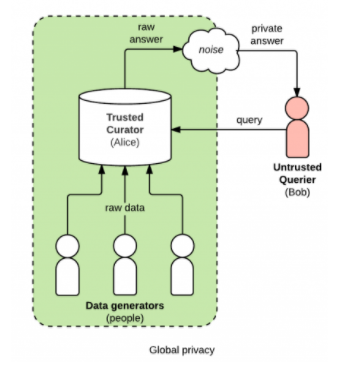
\includegraphics[scale=0.5]{TrustedCuratorModel.png}
        %\caption{Trusted curator model}
        \label{fig:trusted}
\end{figure}
\end{frame}

\begin{frame}{Definitions}
\begin{definition}
\textbf{Neighbouring Datasets: }Two datasets $X$ and $X^\prime$ are said to be neighbouring datasets if they differ only in one row.
\end{definition}
\pause
\begin{definition}
\textbf{$\epsilon$-differential privacy: }Let $X$, $X^\prime \in \mathscr{X}^n$ be two neighbouring datasets also denoted by $X \sim X^\prime$ and $M:\mathscr{X}^n \rightarrow \mathscr{Y}$ be an algorithm said to be $\epsilon$-differentially private, if for all neighbouring  datasets $X$, $X^\prime$ and for all $T \subseteq \mathscr{Y}$,
$$Pr[M(X) \in T] \leq e^\epsilon Pr[M(X^\prime) \in T]$$
Where $\mathscr{X}^n$ and $\mathscr{Y}$ is the set of all datasets and set of all queries respectively. This definition is due to Dwork, McSherry, Nissim and Smith in 2006.
\end{definition}

\end{frame}

\begin{frame}
\textbf{Some Points on the definition of differential privacy: }
\begin{itemize}
\item
$\epsilon$-differential privacy is quantitative in nature. \pause
\item
Small value of $\epsilon$ implies strong privacy. \pause
\item
Grantees privacy at an individual label. Thus by its nature it provides privacy for all $X \sim X^\prime$. Hence privacy of outliers are protected. \pause
\item
For small value of $\epsilon$, $e^\epsilon \simeq (1+\epsilon)$. So for small value of $\epsilon$ here we can visualise that both probabilities are very close on neighbouring databases. \pause
\item
The fact $e^{\epsilon_1} . e^{\epsilon_2}=e^{\epsilon_1 + \epsilon_2}$, is helpful when we consider group privacy. \pause
\item
The definition is symmetric, hence the role of the both datasets $X$ and $X^\prime$ can be interchanged. \pause
\end{itemize}
\end{frame}

\begin{frame}{Properties: Post-Processing}
\begin{theorem}
If $M:\mathscr{X}^n \rightarrow \mathscr{Y}$ be $\epsilon$-differentially private mechanism, and if $G:\mathscr{Y} \rightarrow \mathscr{Z}$ be any randomized mapping then $M \circ G$ is a $\epsilon$-differentially private mechanism.
\end{theorem}
\pause
\begin{proof}
$G$ is a randomized function, we can consider it to de distributed uniformly over all deterministic function g. Now consider $X, \: X^\prime$ are two neighbouring databases and $T \subseteq \mathscr{Y}$,
$$Pr[G(M(X)) \in T]$$
$$=\mathbb{E}_{g \sim G}[Pr[M(X) \in g^{-1}(T)]]$$ 
$$\leq \mathbb{E}_{g \sim G}[e^\epsilon Pr[M(X^\prime) \in g^{-1}(T)]]$$
$$=e^\epsilon Pr[G(M(X^\prime)) \in T]$$
Hence the proof.
\end{proof}
\end{frame}


\begin{frame}[allowframebreaks]{Properties: Group Privacy}
\begin{theorem}
If $M:\mathscr{X}^n \rightarrow \mathscr{Y}$ be $\epsilon$-differentially private mechanism, and $X, \: X^\prime$ are two neighbouring databases, such that they differ in exactly $k$-positions. Then $\forall T \subseteq \mathscr{Y}$,
$$Pr[M(X) \in T] \leq e^{k\epsilon} Pr[M(X^\prime) \in T$$
\end{theorem}

\begin{small}
\begin{proof}
Since the data bases $X, \: X^\prime$ differ in k position so there should exist intermediate databases which differ in exactly one row. so we define $X=X_0, X_1, \dots ,X^\prime=X_k$ a sequence of databases each has an extra row from the former database.\\
Then $\forall T \subseteq \mathscr{Y}$ we have,
$$Pr[M(X) \in T]=Pr[M(X_0) \in T]$$
$$\leq e^\epsilon Pr[M(X_1) \in T]$$
$$\leq e^{2\epsilon} Pr[M(X_2) \in T]$$
$$\dots$$
$$\leq e^{k\epsilon} Pr[M(X_k) \in T]$$
$$= e^{k\epsilon} Pr[M(X^\prime) \in T]$$
Hence the proof.
\end{proof}
\end{small}
\end{frame}


\begin{frame}[allowframebreaks]{Properties: Group Privacy}
\begin{theorem}
Let us consider $M=(M_1, M_2, \dots, M_k)$ is a sequence of $\epsilon$-differentially private mechanism, may have been chosen adaptively then, $M$ is $k\epsilon$-differentially private.
\end{theorem}

\begin{proof}
Let us take two fixed databases $X, \: X^\prime$, also a sequence of outputs $y=(y_1, y_2, \dots, y_k)$. We have the following,
$$\frac{Pr[M(X)=y]}{Pr[M(X^\prime)=y]}$$
$$=\prod_{i=1}^{k} \frac{Pr[M_i(X)=y_i|(M_1(X), M_2(X), \dots, M_{i-1}(X))=(y_1, y_2, \dots, y_{i-1})]}{Pr[M_i(X^\prime)=y_i|(M_1(X^\prime), M_2(X^\prime), \dots, M_{i-1}(X^\prime))=(y_1, y_2, \dots, y_{i-1})]}$$
$$\leq \prod_{i=1}^{k} \exp(\epsilon)$$
$$=exp(k\epsilon)$$
Hence the proof.
\end{proof}
\end{frame}

\begin{frame}[allowframebreaks]{Relationship with Hypothesis testing}
Let output $Y$ is generated from some differentially private mechanism $M$ operating on some $X \sim X^\prime$. An adversary wants to distinguish,
\[
  \begin{cases}
                      H_0: Y \: came \: from \: X \\
                      H_1: Y \: came \: from \: X^\prime
  \end{cases}
\]
Now in statical set-up we may consider this as a hypothesis testing. Now intuitively differential privacy grantees that the adversary will not have any significant advantage than random guessing.\\
Now consider
\[
  \begin{cases}
                      p:= Pr[Adversay \: predicts \: H_1|H_0 \: true] \\
                      q:= Pr[Adversay \: predicts \: H_0|H_1 \: true]
  \end{cases}
\]
i.e. probability of false positive and false negative respectively.\\
Now $\epsilon$ differential privacy simultaneously impels that,
\[
  \begin{cases}
                      p+e^\epsilon q \geq 1 \\
                      pe^\epsilon + q \geq 1
  \end{cases}
\]
The above equation is due to Wasserman and Zhou [Ref 3].\\
This equitations intuitively tells that when $\epsilon=0$, the advantage is also most negligible from blind guessing. But as the $\epsilon$ increases the adversary has an advantage rather than blind guessing.
\end{frame}


%\section{Laplace Distribution}
\begin{frame}
\begin{center}
\Huge \tcr{Laplace Distribution}
\end{center}
\begin{figure}[!ht]
        \centering
        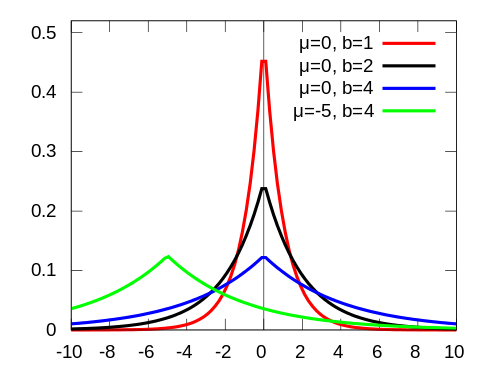
\includegraphics[scale=0.5]{Laplace.png}
        \label{fig:lap}
\end{figure}
\end{frame}


\begin{frame}{Laplace distribution}
\begin{definition}
\textbf{Laplace Distribution:}The density of Laplace distribution with location and scale parameter $\mu, b$ is given by
$$p(x)=\frac{1}{2b}\exp{\{-\frac{|x-\mu|}{b}\}}$$
\end{definition}

\textbf{Some properties of exponential distribution}
\begin{itemize}
\item
It is symmetric about its scale parameter, if scale $\mu=0$ it is symmetric about 0.
\item
It has variance $2b^2$
\item
Tail probability of Laplace distribution is proportional to $\exp{\{-k|x|\}}$. So its probability is concentrated towards centre and it has decaying tail.
\end{itemize}
\end{frame}



%\section{Laplace Mechanism}
\begin{frame}
\begin{center}
\Huge \tcr{Laplace Mechanism}
\end{center}
\begin{figure}[!ht]
        \centering
        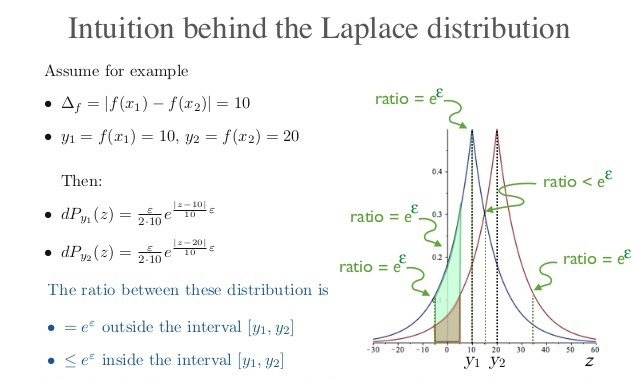
\includegraphics[scale=0.5]{LaplaceIntution.jpg}
        \label{fig:lap}
\end{figure}
\end{frame}



\begin{frame}{Laplace Mechanism}
\begin{small}
\begin{definition}
\textbf{$l_1$ sensitivity: }Consider $f:\mathscr{X}^n \rightarrow \mathbb{R}^k$. The $l_1$ sensitivity of f is
$$\Delta_f= \max_{X, X^\prime} \norm{f(X)-f(X^\prime)},$$
where $X$ and $X^\prime$ are neighbouring data bases and $\norm{.}$ is $l_1$ norm.
\end{definition}
\pause

\tcr{\textbf{Why sensitivity?}}
\pause
Main object of differential privacy is to preserve individuals privacy. So sensitivity of a function is the most natural choice to analyse.\pause

\begin{definition}
\textbf{Laplace Mechanism: }Consider $f:\mathscr{X}^n \rightarrow \mathbb{R}^k$. Then Laplace mechanism is defined as
$$M(X)=f(X)+(Y_1,Y_2,\dots,Y_k),$$
where the $Y_i$ are independent Laplace$(\frac{\Delta}{\epsilon})$ random variables.
\end{definition}
\end{small}
\end{frame}


\begin{frame}[allowframebreaks]{Laplace Mechanism is differentially private}
\begin{theorem}
\label{th1}
The Laplace mechanism is $\epsilon$-differentially private.
\end{theorem}

\begin{proof}
Consider two neighbouring databases $X$ and $Y$, also assume that $p_X$ and $p_Y$ be two pdfs corresponding to $M(X)$ and $M(Y)$ over the support $\mathbb{R}^k$.
$$\frac{p_X(z)}{p_Y(z)}=\frac{\prod_{i=1}^{k} \exp(- \frac{\epsilon |f(X)_i - z_i}{\Delta})}{\prod_{i=1}^{k} \exp(- \frac{\epsilon |f(Y)_i - z_i|}{\Delta})}$$

$$=\prod_{i=1}^{k} \exp(- \frac{\epsilon (|f(X)_i - z_i| - |f(Y)_i - z_i| )}{\Delta})\leq \prod_{i=1}^{k} \exp(- \frac{\epsilon (|f(X)_i - f(Y)_i| )}{\Delta})$$

$$=\exp(- \frac{\sum_{i=1}^{k} \epsilon (|f(X)_i - f(Y)_i| )}{\Delta})=\exp(- \frac{ \epsilon \norm{f(X)_i - f(Y)_i}}{\Delta})\leq \exp(- \epsilon)$$

The third lines follows from triangle inequality, and the last line follows using the definition of $l_1$ sensitivity of a function.
\end{proof}
\end{frame}


\begin{frame}[allowframebreaks]{An example}
\tcr{Effect of $\epsilon$-differential privacy on mean function.}

Consider the mean function,
$$f=\sum_{i=1}^{k} X_i; \: X_i \in \{0,1\}$$
Here we are considering $X_i$'s as indicator variable of a person's habit. Clearly the sensitivity of function $f$ will be $\Delta=\frac{1}{n}$ because presence and absence of a person will contribute 1 in the numerator.\\
Now if we want estimate $p$ the ratio of persons having that habit in the database the by Laplace mechanism we have
$$\hat{p}=f(X) + Y$$
Where $Y$ is a is Laplace$(\frac{\Delta}{\epsilon})$ random variable and $X$ is the $k$-tuple vector. Now $(\frac{\Delta}{\epsilon}) = (\frac{1}{n\epsilon})$.

Now, we observe that $\mathbb{E}(Y)=0$, sine location parameter is zero. Also $p=f(X)$ the original ratio from the database. Therefore we have,

$$\mathbb{E}(\hat{p}) = p$$

\begin{definition}
\textbf{Tchebychev's inequality}If $X$ is a RV with finite expectation $\mu$ and variance $\sigma^2 \geq 0$ the for all real number $k > 0$,
$$Pr[|X- \mu| \leq k\sigma] \geq 1 - \frac{1}{k^2}$$
\end{definition}

Let us calculate variance of $\hat{p}$,

$$Var[\hat{p}]= Var[Y + f(X)]$$
$$=Var[Y] $$
$$=\frac{1}{\epsilon^2 n^2}$$
Now if we apply Tchebychev's inequality with the random variable as $\hat{p}$ we get,
$$Pr[|\hat{p}- p| \leq \frac{k}{n\epsilon}] \geq 1 - \frac{1}{k^2};\: \forall k > 0$$
That is we have,
$$|\hat{p}- p| \leq \mathcal{O}(\frac{1}{n\epsilon})$$
with reasonable probability, and also it differentially private since Laplace mechanism is differentially  private.
\end{frame}


\begin{frame}[allowframebreaks]{Counting query \& Histogram query}
\tcr{\textbf{Single counting query: }}In a database there is a binary column $P$, corresponds to a property entries of database[each row]. We want to know $f=\sum_{i} X_i$, $X_i \in \{0,1\}$ if $i^{th}$ row has property $P$. So here $f(X)+ Laplace(\frac{1}{\epsilon})$ is the privatization statistic, With error $\mathcal{O} (\frac{1}{\epsilon})$.\\

\tcr{\textbf{Multiple counting query: }}Consider $k$ counting query, $f=(f_1,f_2, \dots, f_k)$, which are fixed before[non-adaptive]. $f(X)+ Y$ will be privatization statistic. Where $Y=(Y_1,Y_2, \dots, Y_k)$ are independent Laplace random variables.\\ 
\tcr{\textbf{Which scale parameter should we use?}} Each query $f_i$ has sensitivity 1[as counting query], and the underlying database is same so changing an individual person will change the result of many counting queries.\\
Lets take an example consider two persons one has no properties another has all the properties, changing them will cause $l_1$ sensitivity to differ by $k$. So in this case the sensitivity is bounded by
$$\Delta_f=\sum_{i} |f_i(X)-f_i(X^\prime)| \leq k,$$
where $X, X^\prime$ are neighbouring databases. Thus we will use $\Delta=k$ and we will add noise $Y_i \sim Laplace(k/\epsilon)$ into each co-ordinates.


\tcr{Histogram query} is example of a structured query. Where each universe $\mathscr{X}^n$ is partitioned into bins. So a person, at a time can belong to a single bin. Due to the above fact addition of one individual will change, the count of histogram query at most 1, this type of queries can be answered by adding independent draws from $Laplace(1/\epsilon)$ to the original count of each cell.
\end{frame}




%\section{Exponential Mechanism}
\begin{frame}
\begin{center}
\Huge \tcr{Exponential Mechanism}
\end{center}
\begin{figure}[!ht]
        \centering
        \label{fig:lap}
\end{figure}
\end{frame}


\begin{frame}{Motivation beyond Exponential Mechanism}
The exponential mechanism was designed for cases where we wish the best response, but adding some noise to the best value can dramatically change the its value.\\
Consider example of an auction where auction house has adequate supply of a product, and we have \tcr{3 bider} they wants to bid on the product \tcr{first two bider are willing to pay \$1} and \tcr{third bidder willing to pay \$3.01} for the product. Now consider the following situations,
\begin{itemize}
\item
Price at the auction house is \$1 in this case revenue will be \$3.
\item
Price at the auction house is \$1.01 in this case revenue will drop to \$1.01.
\item
Price at the auction house is \$3.01 in this case revenue will be \$3.01.
\item
Price at the auction house is \$3.02 in this case revenue will be \$0.
\item
We can see that dramatic change in revenue in 2 and 4th point. While the change of price is very few. Hence here sensitivity is more.
\item
So here instead considering prices as numerical value we will consider prices as objects. So in this set up price \$1 and \$3.01 as ``High quality object" and 1.01 and 3.02 as ``Low quality object"
\end{itemize} 
\end{frame}

\begin{frame}{Definition: Exponential Mechanism}
Consider,a dataset $X \in \mathscr{X}^n$, a set of objects $\mathscr{H}$ \& a score function $s:\mathscr{X}^n \times \mathscr{H} \rightarrow \mathbb{R}$


\begin{definition}
\textbf{Sensitivity of the score function} for two neighbouring dataset $X, X^\prime$ is defined as,
$$\Delta_s = \max_{h \in \mathscr{H}} \max_{X, X^\prime} \norm{s(X,h)-s(X^\prime,h)},$$ 
\end{definition}

\begin{definition}
The exponential mechanism $M_E(X,h,s)$ selects and outputs some object $h \in \mathscr{H}$, with probability proportional to $\exp(\frac{\epsilon s(X,h)}{2\Delta})$.
\end{definition}

\textbf{Note: We assume that set of objects and the score function are public and we don't bother about their security or privacy. The only is the dataset $X$ which is kept secret here.}\\
Thus sensitivity of the score function is defined on the dataset only.
\end{frame}



\begin{frame}[allowframebreaks]{Privacy proof}
\begin{small}
\begin{theorem}
The exponential mechanism $M_E$ is $\epsilon$-differentially private mechanism.
\end{theorem}

\begin{proof}
Let us fix two neighbouring datasets $X, X^\prime$ and some $h \in \mathscr{H}$, Then we have
$$\frac{Pr[M_E(X)=h]}{Pr[M_E(X^\prime)=h]}=\frac{\frac{\exp(\frac{\epsilon s(X,h)}{2\Delta})}{\sum_{h^\prime} \exp(\frac{\epsilon s(X,h^\prime)}{2\Delta})}}  {\frac{\exp(\frac{\epsilon s(X^\prime,h)}{2\Delta})}{\sum_{h^\prime} \exp(\frac{\epsilon s(X^\prime,h^\prime)}{2\Delta})}}=exp(\frac{\epsilon (s(X,h) - s(X^\prime,h))}{2\Delta})  \frac{\sum_{h^\prime} \exp(\frac{\epsilon s(X^\prime,h^\prime)}{2\Delta})}{\sum_{h^\prime} \exp(\frac{\epsilon s(X,h^\prime)}{2\Delta})}$$

$$\leq \exp(\epsilon/2) \exp(\epsilon/2) \frac{\sum_{h^\prime} \exp(\frac{\epsilon s(X,h^\prime)}{2\Delta})}{\sum_{h^\prime} \exp(\frac{\epsilon s(X,h^\prime)}{2\Delta})}=\exp(\epsilon)$$

The above inequality holds based on the definition of $\Delta$ that,
$$\exp(\frac{\epsilon s(X^\prime,h^\prime)}{2\Delta}) \leq \exp(\epsilon/2) \exp(\frac{\epsilon s(X,h^\prime)}{2\Delta})$$
Hence the proof.
\end{proof}
\end{small}
\end{frame}



\begin{frame}{Connection between Exponential and Laplace Mechanism}
\subsection{Relation between Exponential and Laplace Mechanism}
Laplace mechanism can be thought as a particular case of exponential mechanism. Lets take we are interested in computing the sensitivity of $\Delta$ statistic $f:\mathscr{X}^n \rightarrow \mathbb{R}$ on a dataset $X$ by Laplace mechanism.\\
Now let us take set of objects $\mathscr{H}$ is the real line $\mathbb{R}$, and the score function $s(X,h)=-|f(X)-h|$.\\
This yields the probability of a point $h \in \mathbb{R}$ being output with probability proportional to $\exp(-\frac{\epsilon|f(X)-h|}{2\Delta})$. Which is exactly the density of Laplace distribution upto a factor 2, Which can be removed with more care.\\
\end{frame}









\begin{frame}[allowframebreaks]{Approximate Differential Privacy}
Here we will discuss relaxation in the definition $\epsilon$-differential privacy. This relaxation was first proposed by Dwork, Kenthapadi, McSherry, Mironov, and Naor. The main idea for weakening privacy notion is that to achieve it less amount of noise.

\begin{definition}
\textbf{Approximate Differential Privacy} A mechanism $M:\mathscr{X}^n \rightarrow \mathscr{Y}$ is $(\epsilon, \delta)$ differential private, if for all neighbouring datasets $X$, $X^\prime \in \mathscr{X}^n$ and for all $T \subseteq \mathscr{Y}$,
$$Pr[M(X) \in T] \leq e^\epsilon Pr[M(X^\prime) \in T] + \delta$$
\end{definition}
To interpret new definition we will require another notion, called \textbf{privacy loss random
variable}.
 
\begin{definition}
Let $Y$ and $Z$ be two random variables, then a privacy loss random variable $\mathscr{L}_{Y||Z}$ is distributed by drawing $t \sim Y$, and outputting $\ln{\frac{Pr[Y=t]}{Pr[Z=t]}}$.
\end{definition}
\textbf{Remark 1: }In the above definition supports of Y and Z are should be equal, otherwise the privacy loss random variable is undefined. In fact this holds for continuous random variables also.\\
\textbf{Remark 2: }We have defined privacy loss in terms of random variables but we will apply it as for $Y, Z$ equal to $M(X)$ and $M(X^\prime)$ where $X \sim X^\prime$ are two neighbouring datasets.\\
Intuition behind notion of privacy loss random variable is that how much it is likely to be input database is $X$ compared to $X^\prime$ based on the observation of the realization of $M(X)$.
\end{frame}










%\section{R implementation}
\begin{frame}
\begin{center}
\Huge \tcr{R implementation}
\end{center}
\begin{figure}[!ht]
        \centering
        \label{fig:lap}
\end{figure}
\end{frame}


\begin{frame}[fragile]{R implementation of Laplace Mechanism}
\begin{lstlisting}[language=R]
# Here we will demonstrate Laplace privatization of
# the sample mean on bounded data [0,1]
library(diffpriv)
func <- function(X) mean(X) ## target function
n <- 150 ## dataset size
mechanism <- DPMechLaplace(target = func, sensitivity = 1/n, dims = 1)
Database <- runif(n, min = 0, max = 1) ## the sensitive database in [0,1]^n
pparams <- DPParamsEps(epsilon = 1) ## desired privacy budget
r <- releaseResponse(mechanism, privacyParams = pparams, X = Database)
cat("Private response r$response:", r$response,
    "\nNon-private response f(D): ", func(Database))
\end{lstlisting}

Output we get
\begin{verbatim}
Private response r$response: 0.4688349 
Non-private response f(D):  0.4733297
\end{verbatim}
\end{frame}


\begin{frame}[fragile, allowframebreaks]{R implementation of Exponential Mechanism}
\begin{lstlisting}[language=R]
# we demonstrate the exponential mechanism here

library(randomNames) ## a package that generates representative random names
oracle <- function(n) randomNames(n)
Database <- c("Cust A", "Cust B", "Cust C","Cust D",
       "Cust E", "Cust F", "Cust G",
       "Cust H", "Cust I", "Cust J")
n <- length(Database)
func <- function(X) { function(r) sum(r == unlist(base::strsplit(X, ""))) }
rSet <- as.list(letters) ## the response set, letters a--z, must be a list
mechanism <- DPMechExponential(target = func, responseSet = rSet)
# 
mechanism <- sensitivitySampler(mechanism, oracle = oracle, n = n, gamma = 0.1)
pparams <- DPParamsEps(epsilon = 1)
r <- releaseResponse(mechanism, privacyParams = pparams, X = Database)
cat("Private response r$response: ", r$response,
    "\nNon-private f(D) maximizer: ", letters[which.max(sapply(rSet, func(Database)))])
\end{lstlisting}

Output we get
\begin{verbatim}
Private response r$response:  j 
Non-private f(D) maximizer:  b>
\end{verbatim}
\end{frame}


\begin{frame}{References}
\begin{enumerate}
\item
Calibrating Noise to Sensitivity in Private Data Analysis. Cynthia DworkFrank McSherryKobbi NissimAdam Smith.
\item
The Composition Theorem for Differential Privacy, Peter Kairouz, Sewoong Oh, Pramod Viswanath.
\item
A statistical framework for differential privacy. Larry Wasserman, Shuheng Zhou.
\item
Revealing Information while Preserving Privacy. Irit Dinur,  Kobbi Nissim.
\item
The Algorithmic Foundations of Differential Privacy. Aaron Roth and Cynthia Dwork.
\item
Our Data, Ourselves: Privacy Via Distributed Noise Generation. Cynthia Dwork, Krishnaram Kenthapadi, Frank McSherry, Ilya Mironov, Moni Naor.
\end{enumerate}
\end{frame}








\end{document}